\section{Algorithm Selection Problem}

Das \textit{Algorithm Selection Problem} (ASP), bereits 1976 von John Rice formuliert \cite{rice76}, be"-schäftigt sich mit der Frage, welchen Algorithmus man zur Berechnung der Lösung eines Problems am ehesten benutzen sollte. Obwohl das Problem einfach beschrieben werden kann ergeben sich daraus viele schwierige Fragestellungen. Dieser Abschnitt soll einen kurzen Überblick über einige dieser Fragen geben.

Rice betrachtet unterschiedliche Mengen um das ASP zu charakterisieren (siehe Abbildung \ref{asp}). Eine davon ist die Problemmenge $\mathcal{P}$. Im Bereich der Simulation könnten unter anderem verschiedene Modelle innerhalb dieser Menge sein. Denkbar wäre zum Beispiel das Problem der Berechnung einer Zustandsüberführung eines zellulären Automaten.

Anhand dieser Probleme unterscheidet Rice nun drei Arten das ASP zu lösen. Man sucht einen Algorithmus, der entweder für alle Probleme oder für eine bestimmte Problemklasse oder nur für ein einzelnes Problem der beste Algorithmus ist. Universell beste Algorithmen zu finden ist dabei eine nicht realistisch zu lösende Aufgabe \cite{smith09}. Ideale Algorithmen für Problemklassen zu finden ist die interessante Variante des ASP.

Schwierigkeiten bei diesem Ansatz bereitet die Definition der Problemklassen. Es müssen Eigenschaften, dargestellt in der Eigenschaftsmenge $\mathcal{E}$, gefunden werden, welche Probleme zu Klassen zusammenfassen und gleichzeitig folgendes Kriterium erfüllen: Erzielt ein Algorithmus gute Ergebnisse für ein Problem einer Problemklasse, dann muss er auch gute Ergebnisse für alle anderen Probleme dieser Klasse liefern. 

Das Finden von repräsentativen Eigenschaften für Problemklassen wird von Rice als eine der am wichtigsten zu lösenden Aufgaben des ASP bezeichnet und ist heute als eigenständiges Problem unter dem Namen \textit{Feature Selection Problem} bekannt \cite{kira92, guyon03}. 


Alleine die Tatsache, dass ein Algorithmus abhängig von den Parametern eines einzelnes Problems gute oder schlechte Ergebnisse liefern kann \cite{roberts06}, unterstreicht die Schwierigkeit einer geeigneten Klassifizierung. Zudem gibt es dynamische Eigenschaften, welche erst zur Laufzeit berechnet werden können. Wie sollen solche Eigenschaften vor der Ausführung der Algorithmen zur Konstruktion der Problemklassen benutzt werden? 

Bei Simulationsmodellen scheint eine mögliche Einteilung auf den ersten Blick einfach: eine Modellart entspricht einer Problemklasse. Jedoch kann auch ein Modelltyp unterschiedliche Varianten aufweisen. Je nachdem ob zum Beispiel zelluläre Automaten deterministisch sind oder stochastische Elemente enthalten müssen Eigenschaften anders bewertet werden. Des Weiteren muss auch die Hardware, auf der das Modell ausgeführt werden soll, bei der Bewertung der Eigenschaften mit berücksichtigt werden.

Neben der Problem- und Eigenschaftsmenge muss die Algorithmenmenge $\mathcal{A}$ betrachtet werden. Im Idealfall sollte diese Menge möglichst viele Lösungsalgorithmen für eine Problemklasse enthalten, jedoch ist die Analyse dieser dann sehr großen Menge von Algorithmen zu aufwändig, sodass die Algorithmenmenge eingeschränkt werden muss. Das führt zwangsweise dazu, dass eine Art Vorauswahl getroffen werden muss. Fehler bei dieser Vorauswahl lassen sich nicht vermeiden, sodass gute Algorithmen möglicherweise von vornherein ausgeschlossen werden. 

Auch bei Simulationsproblemen kann die Algorithmenmenge sehr groß sein. Ein Beispiel für einen solchen Fall ist das Modellierungs- und Simulationsframework JAMES II, welches die Möglichkeit bietet Algorithmen zu kombinieren. Durch die möglichen Kombinationen steigt die Anzahl der Algorithmen in der Algorithmenmenge stark an \cite{ewald10}.

Abschließend führt Rice die Notwendigkeit einer Metrik zur Bewertung der Algorithmen an. Um sie zu definieren müssen geeignete Eigenschaften und ein zweckmäßiges Verhältnis für die Bewertung zwischen diesen Eigenschaften gefunden werden. Beispiele für solche Eigenschaften sind die Laufzeit- und Platzkomplexität, die Optimalität eines Ergebnisses oder die Einfachheit eines Algorithmus. Die erhaltenen Ergebnisse der Leistungsmessung können dann im Performanceraum $\mathcal{Y}$ abgebildet werden, welcher die Leistung eines Algorithmus für ein bestimmtes Problem bestimmt.
 \\


\begin{figure}[h]
\centering
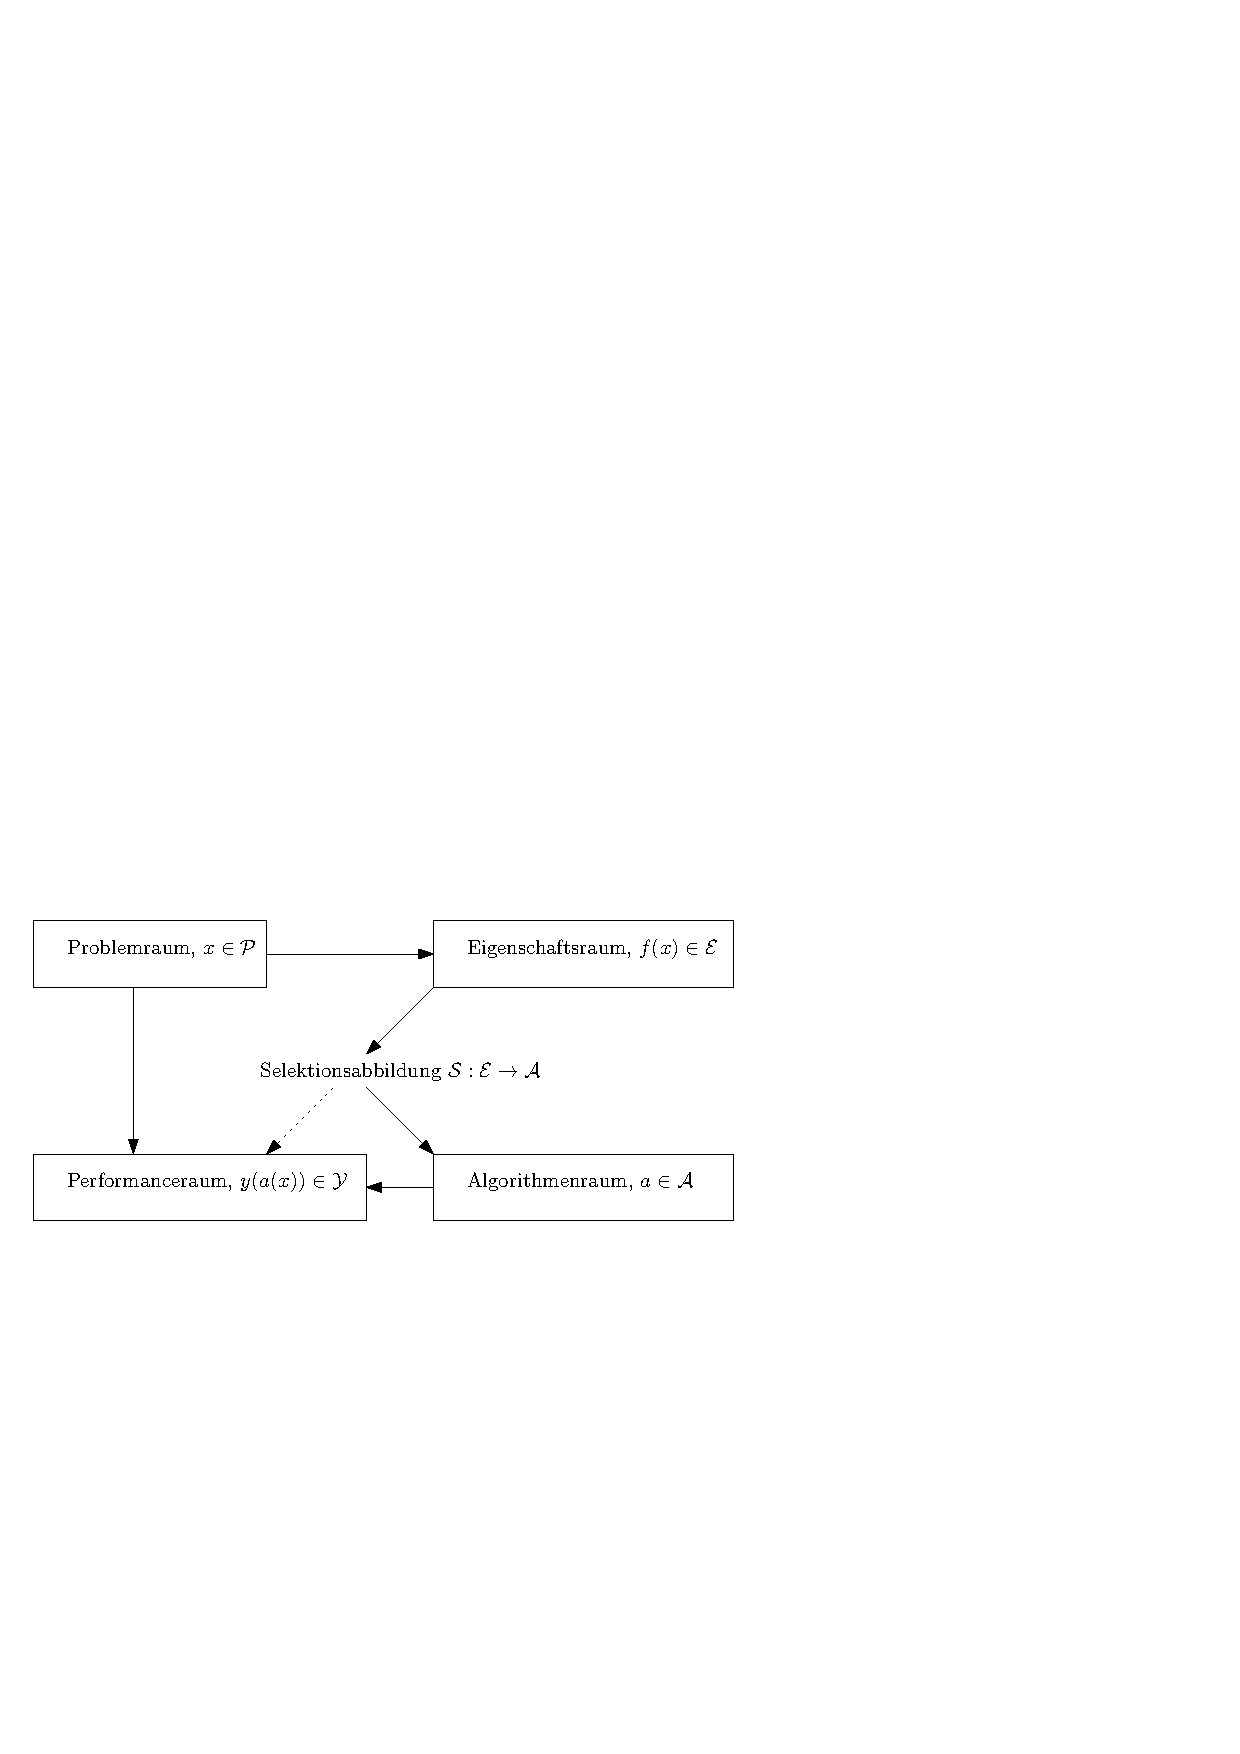
\includegraphics{asp.pdf}
\caption[Algorithm Selection Problem]{Charakterisierende Mengen für das \textit{Algorithm Selection Problem}. Eine optimale Selektionsabbildung $\mathcal{S}$ ist gesucht, welche folgende Eigenschaft erfüllt: $a = S(f(x)) \Rightarrow y(a(x)) = max(y(\alpha (x)) $~$ \forall \alpha \in \mathcal{A}$}
\label{asp}
\end{figure}

